\section{Background} \label{sec:2background}

\subsection{Entropy and Brute-Force Attacks}

Entropy was introduced by Shannon~\cite{shannon1948communicationtheory} to quantify the randomness and uncertainty within a system.
In the domain of cryptography, the entropy of a key serves as a crucial metric for assessing its strength.

The method of enumerating all possible keys until the correct one is found is called a brute-force attack, which can be classified as either an online or an offline attack.
In an online attack, the adversary persistently sends the attempted keys to the target system to verify their correctness.
In an offline attack, the attacker need only obtain the ciphertext and test all possible keys to decrypt it.
% Since online attacks require continuous interaction with the target system, they are less efficient than offline attacks.
In this paper, we focus on offline brute-force attacks; all subsequent references to brute-force attacks refer to the offline variant unless stated otherwise.

\subsection{Protocols Tolerating Low-Entropy Keys}
Low-entropy keys are common in practice.
Backward compatibility, power consumption constraints, and user experience requirements prevent many protocols from guaranteeing high-entropy keys for all cryptographic variables.
We examine three representative protocols: WPA2-PSK, Bluetooth Low Energy (BLE), and Bluetooth Classic (BC).

\subsubsection{WPA2-PSK}
Wi-Fi Protected Access 2 Pre-Shared-Key~(WPA2-PSK) establishes a secure connection between a supplicant and an authenticator in a personal Wi-Fi network.
\autoref{fig:4-way-handshake} illustrates the protocol, where both parties derive a Pairwise Transient Key~$PTK$ from a Pairwise Master Key~$PMK$, which is computed from a pre-shared $Passphrase$ and the network name~$SSID$:
\begin{equation} \label{eq:pmk}
    PMK = \text{PBKDF2}(Passphrase, SSID)
\end{equation}

\begin{figure}[t]
    \centering
    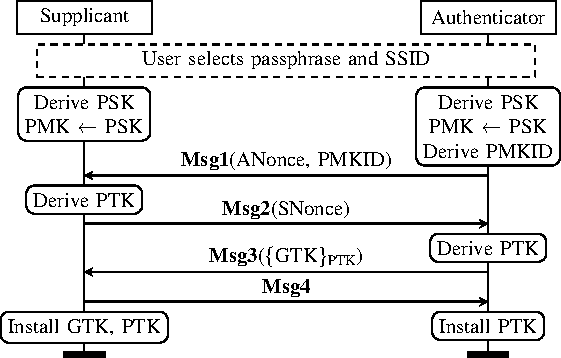
\includegraphics[width=0.870780\columnwidth]{img/4-way-handshake}
    \caption{Overview of WPA2-PSK}
    \label{fig:4-way-handshake}
\end{figure}

The $Passphrase$ consists of 8--63 characters; a user who chooses digits only significantly reduces the entropy of $PMK$.
In the 4-way handshake, the authenticator and supplicant exchange nonces $N_A, N_B$ and derive $PTK = \text{PRF}(PMK, {MAC}_A, {MAC}_S, N_A, N_B)$.
The first EAPOL-key message carries a $PMKID$ field for fast re-authentication, computed as:
\begin{equation} \label{eq:pmkid}
    PMKID = \text{HMAC}(PMK, {MAC}_{A} \| {MAC}_{S})
\end{equation}
Messages~2--4 are protected by a MIC derived from $PTK$, but the $PMKID$ in message~1 is sent before $PTK$ exists and thus lacks integrity protection.
This field is exploited by the PMKID attack~(\S\ref{sec:wpa2-psk}).

\subsubsection{Bluetooth Low Energy~(BLE)}
BLE~\cite{bluetooth4} is designed for short-range, low-power communication.
The BLE pairing protocol negotiates a long-term key~$LTK$ between an initiator and a responder; $LTK$ is then used to derive a session key~$SK$ for an encrypted channel.
\autoref{fig:ble-pairing} shows the pairing process.

\begin{figure}[t]
    \centering
    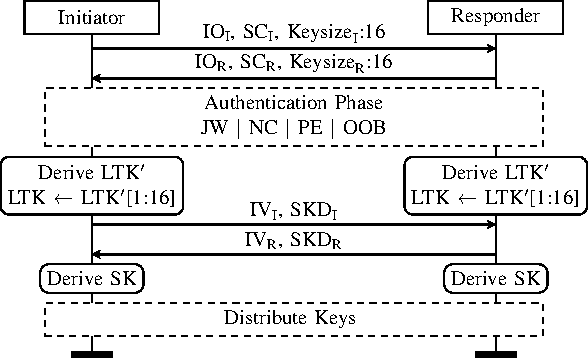
\includegraphics[width=0.912689\columnwidth]{img/ble-pairing}
    \caption{Overview of BLE pairing protocol}
    \label{fig:ble-pairing}
\end{figure}

During feature exchange, devices announce their supported key sizes (7--16 bytes) and IO capabilities.
An intermediate key $LTK'$ is negotiated during authentication, then truncated to the agreed $KeySize$ to form $LTK$.
Both devices then compute $SK = \text{AES-ECB}_{LTK}(SKD_I \| SKD_R)$, where $SKD_I, SKD_R$ are random contributions.
The key-size negotiation and truncation phases are unprotected by integrity checks, enabling an attacker to force a shorter key.

\subsubsection{Bluetooth Classic~(BC)}
Bluetooth Classic (BR/EDR) is designed for high-throughput applications such as audio streaming and file transfer.
\autoref{fig:bc-session} shows the session establishment between paired BC devices.

\begin{figure}[t]
    \centering
    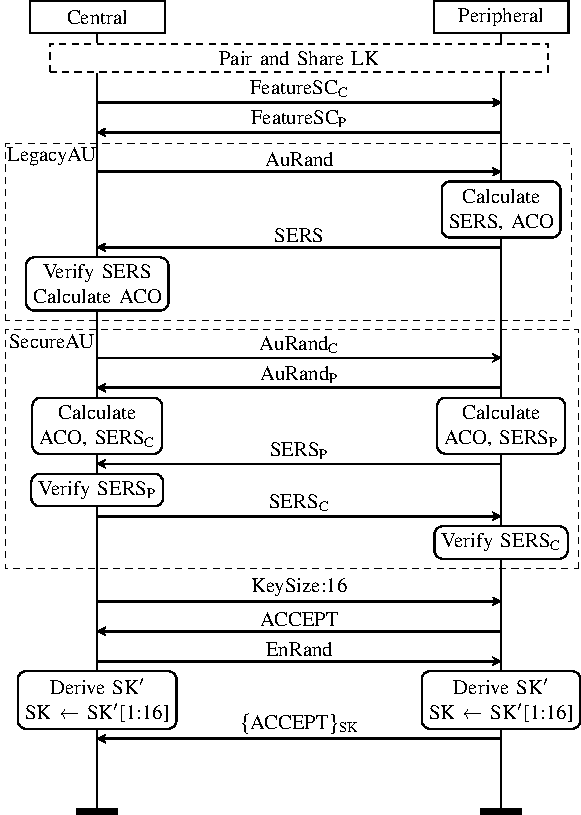
\includegraphics[width=0.902212\columnwidth]{img/bc-session}
    \caption{Overview of BC session establishment protocol}
    \label{fig:bc-session}
\end{figure}

After pairing, both devices share a link key~$LK$.
Session establishment proceeds through four phases: (1)~link connection, where devices exchange supported features including whether they support \emph{Secure Connections}; (2)~authentication, using either Legacy Authentication (unilateral) or Secure Authentication (mutual) to compute an Authenticated Channel Offset~$ACO$ from $LK$ and random values; (3)~key-size negotiation; and (4)~session-key derivation, where the devices compute a session key $SK'$ from $LK$ and $ACO$:
\begin{equation} \label{eq:legacy-sk}
    \text{Legacy:}\; SK' = \text{E3}(LK, EnRand, ACO)
\end{equation}
\begin{equation} \label{eq:secure-sk}
    \text{Secure:}\; SK' = \text{h3}(LK, ACO)
\end{equation}
The final session key~$SK$ is obtained by truncating $SK'$ to the negotiated key length.
The key-size negotiation phase is unprotected, and the encrypted \Tfunction{ACCEPT} message using $SK$ concludes the session establishment.

\subsection{\Tamarin{}}
\Tamarin{}~\cite{meier2013tamarin} is a state-of-the-art tool for formal security protocol verification.
Protocols and adversary behaviors are modeled as labeled multiset rewriting rules of the form $[F_l] \xrightarrow{[F_a]} [F_r]$, where $F_l, F_a, F_r$ are multisets of facts.
A \emph{fact} $F(t_1, \ldots, t_n)$ is built from terms in a term algebra $T_\Sigma(\mathcal{V}, \mathcal{N})$ over function symbols~$\Sigma$, variables~$\mathcal{V}$, and names~$\mathcal{N}$.
Facts are either \emph{linear} (consumed once) or \emph{persistent} (reusable).
\Tamarin{} provides built-in facts \TFact{In} (receive from public channel), \TFact{Out} (send), and \TFact{Fr} (fresh name generation).
Security properties are expressed as first-order trace formulas with time points; for instance, secrecy of a key~$k$ requires that no adversary learns $k$ after it is installed:
\begin{flalign*}
    & \hspace{0em} \TAll \;\, \text{\Tterm{k \#i.}} \;\, \text{\TFact{Install(k)@\#i}} &\\
    & \hspace{3em} \implies \TNot (\TEx \;\, \text{\TLemma{\#j.}} \;\, \text{\TFact{K(k)@\#j}} ) &
\end{flalign*}
